% this file is drba_tp2.tex
% title page
\begin{tabular}{p{\textwidth}}
\begin{flushright}

\includegraphics[scale=0.15]{figures/tuhh.png}
\end{flushright}


\textcolor{gray}{\rule{15cm}{.8pt}}\\
\vspace{0.01cm}
\LARGE{\textsf{\textcolor{blue}{Bachelor Thesis}}} \\
\textcolor{gray}{\rule{15cm}{.8pt}}

~\\
~\\



\begin{center}
\textbf{\LARGE{Daniel Rembold}}
~\\
~\\
~\\
~\\
\textbf{\LARGE{Gröbner Fans for Linear Codes}}
~\\
~\\
~\\
~\\
\textbf{\large{August 2014}}
\end{center}

~\\
\begin{center}
\textcolor{gray}{\rule{15cm}{.8pt}}\\
\vspace{0.1cm}
\begin{tabular}{lll}
\textbf{Advised by:} & & Dipl.-Technomath. Natalia D\"uck \\
\textbf{Supervised by:} & & Prof. Dr. Dr. habil. Karl-Heinz Zimmermann\\
\end{tabular}
\textcolor{gray}{\rule{15cm}{.8pt}}\\
\end{center}

~\\


\begin{wrapfigure}{r}{4cm} % l = Bild wird linksbündig positioniert, möglich ist auch r für rechtsbündig
% 8cm ist der Abstand von links, der für das Bild freigehalten wird, rechts davon kann Text stehen
\centering
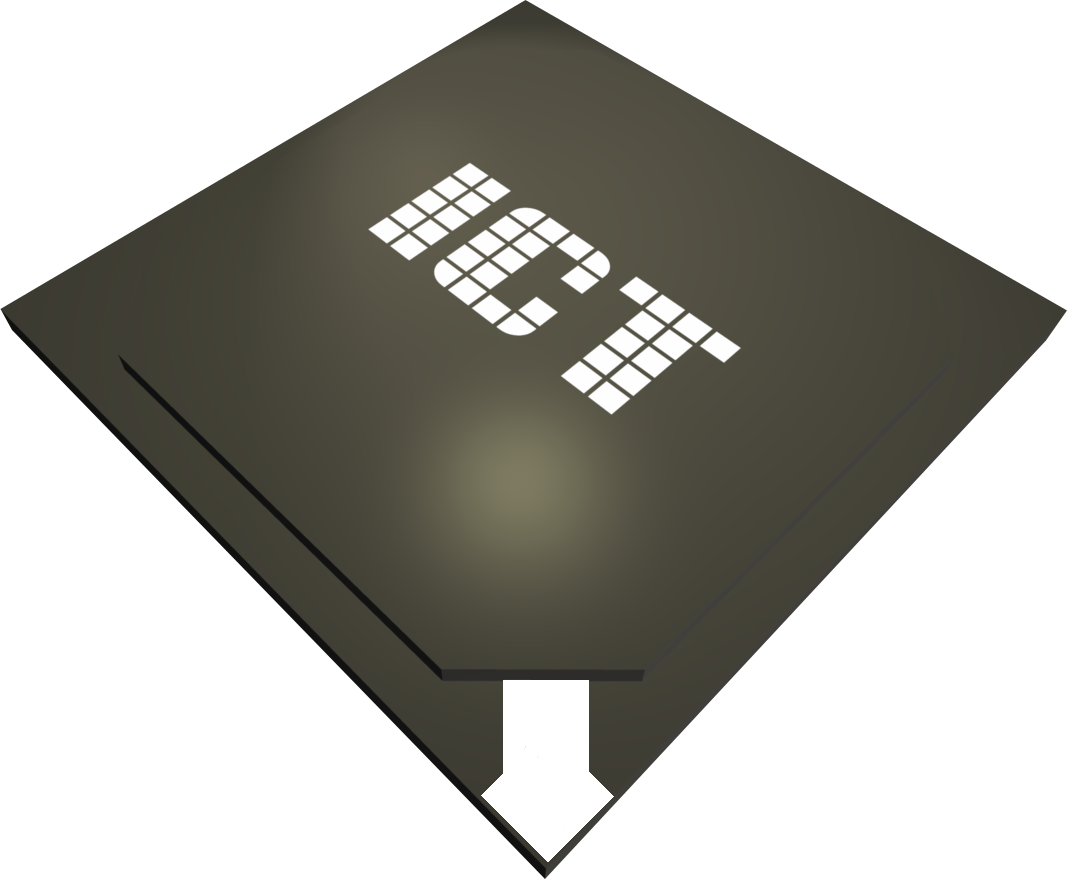
\includegraphics[scale=0.25]{figures/ictlogo.png}
\end{wrapfigure}
Technische Universität Hamburg-Harburg\\
Hamburg University of Technology\\
Institute of Computer Technology (E-13) \\
21071 Hamburg

\end{tabular}


